%\documentclass{book}
\documentclass{article}                            %for shorter notes
\usepackage{graphicx}                              %for PNG images (pdflatex)
%\usepackage{graphics}                              %for EPS images (latex)
\usepackage[linkbordercolor={1.0 1.0 0.0}]{hyperref} %for \url tag
\usepackage{color}                                 %for defining custom colors
\usepackage{framed}                                %for shaded and framed paragraphs
\usepackage{textcomp}                              %for various symbols, e.g. Registered Mark
\usepackage{geometry}                              %for defining page size
\usepackage{longtable}                             %for breaking tables
%
\geometry{verbose,a4paper,tmargin=2.5cm,bmargin=2.5cm,lmargin=2.5cm,rmargin=2cm}
\hypersetup{
  pdfauthor = {Author Name},
  pdftitle = {Paper title},
  pdfsubject = {Paper subject},
  pdfkeywords = {Paper,keyword,comma-separated},
  pdfcreator = {PDFLaTeX with hyperref package},
  pdfproducer = {PDFLaTeX}
}
%
\bibliographystyle{IEEEtran}                       %a nice bibliography style
%
\def\efill{\hfill\nopagebreak}%
\hyphenation{Nordu-Grid}
\setlength{\parindent}{0cm}
\setlength{\FrameRule}{1pt}
\setlength{\FrameSep}{8pt}
\addtolength{\parskip}{5pt}
\renewcommand{\thefootnote}{\fnsymbol{footnote}}
\renewcommand{\arraystretch}{1.3}
\newcommand{\dothis}{\colorbox{shadecolor}}
\newcommand{\globus}{Globus Toolkit\textsuperscript{\textregistered}~2~}
\newcommand{\GT}{Globus Toolkit\textsuperscript{\textregistered}}
\newcommand{\ngdl}{\url{http://ftp.nordugrid.org/download}~}
\definecolor{shadecolor}{rgb}{1,1,0.6}
\definecolor{salmon}{rgb}{1,0.9,1}
\definecolor{bordeaux}{rgb}{0.75,0.,0.}
\definecolor{cyan}{rgb}{0,1,1}
%
%----- DON'T CHANGE HEADER MATTER
\begin{document}
\def\today{\number\day/\number\month/\number\year}

\begin{titlepage}

\begin{tabular}{rl}
\resizebox*{3cm}{!}{\includegraphics{ng-logo.png}}
&\parbox[b]{2cm}{\textbf \it {\hspace*{-1.5cm}NORDUGRID\vspace*{0.5cm}}}
\end{tabular}

\hrulefill

%-------- Change this to NORDUGRID-TECH-NN

{\raggedleft NORDUGRID-TECH-NN\par}

{\raggedleft \today\par}

\vspace*{2cm}

%%%%---- The title ----
{\centering \textsc{\Large ARC Accounting Component -- JURA}\Large \par}
\vspace*{0.5cm}
    
%%%%---- A subtitle, if necessary ----
{\centering \textit{\large Technical document}\large \par}
    
\vspace*{1.5cm}
%%%%---- A list of authors ----
    {\centering \large P\'eter D\'ob\'e \footnote{dobe@iit.bme.hu} \large \par}
    
%%%%---- An abstract - if style is article ----
%\begin{abstract}
%The abstract
%\end{abstract}
\end{titlepage}

%\tableofcontents                          %Comment if use article style
\newpage

\section{Purpose}

The \textit{Job Usage Reporter for ARC} (JURA) is a component
implementing accounting functionality in the ARC middleware. Its
objective is to gather metered resource usage data for each job and
submit it to accounting services along with the job submitter's
identity and miscellaneous job-related metadata.

The accounting service stores the received usage data in a database,
and provides an interface for querying it. Queries can be made by the
consumers of the accounting data, such as a billing component. The
service itself is a third party application, separate from the
middleware distribution. JURA is currently capable of using the
logging service of the SweGrid Accounting System (SGAS)\cite{sgas},
but maintaining the possibility to enable utilizing other services has
been kept in mind during design.

Before the usage data collected from the resource manager is
submitted, it is transformed into records of job-level granularity. To
every job corresponds exactly one Grid user, therefore reports over a
time period (e.g.~an invoice) can be generated per-user, or
alternatively on a larger scale such as job project or VO level.

\section{Architecture}

\begin{figure}[ht]
\centering{{{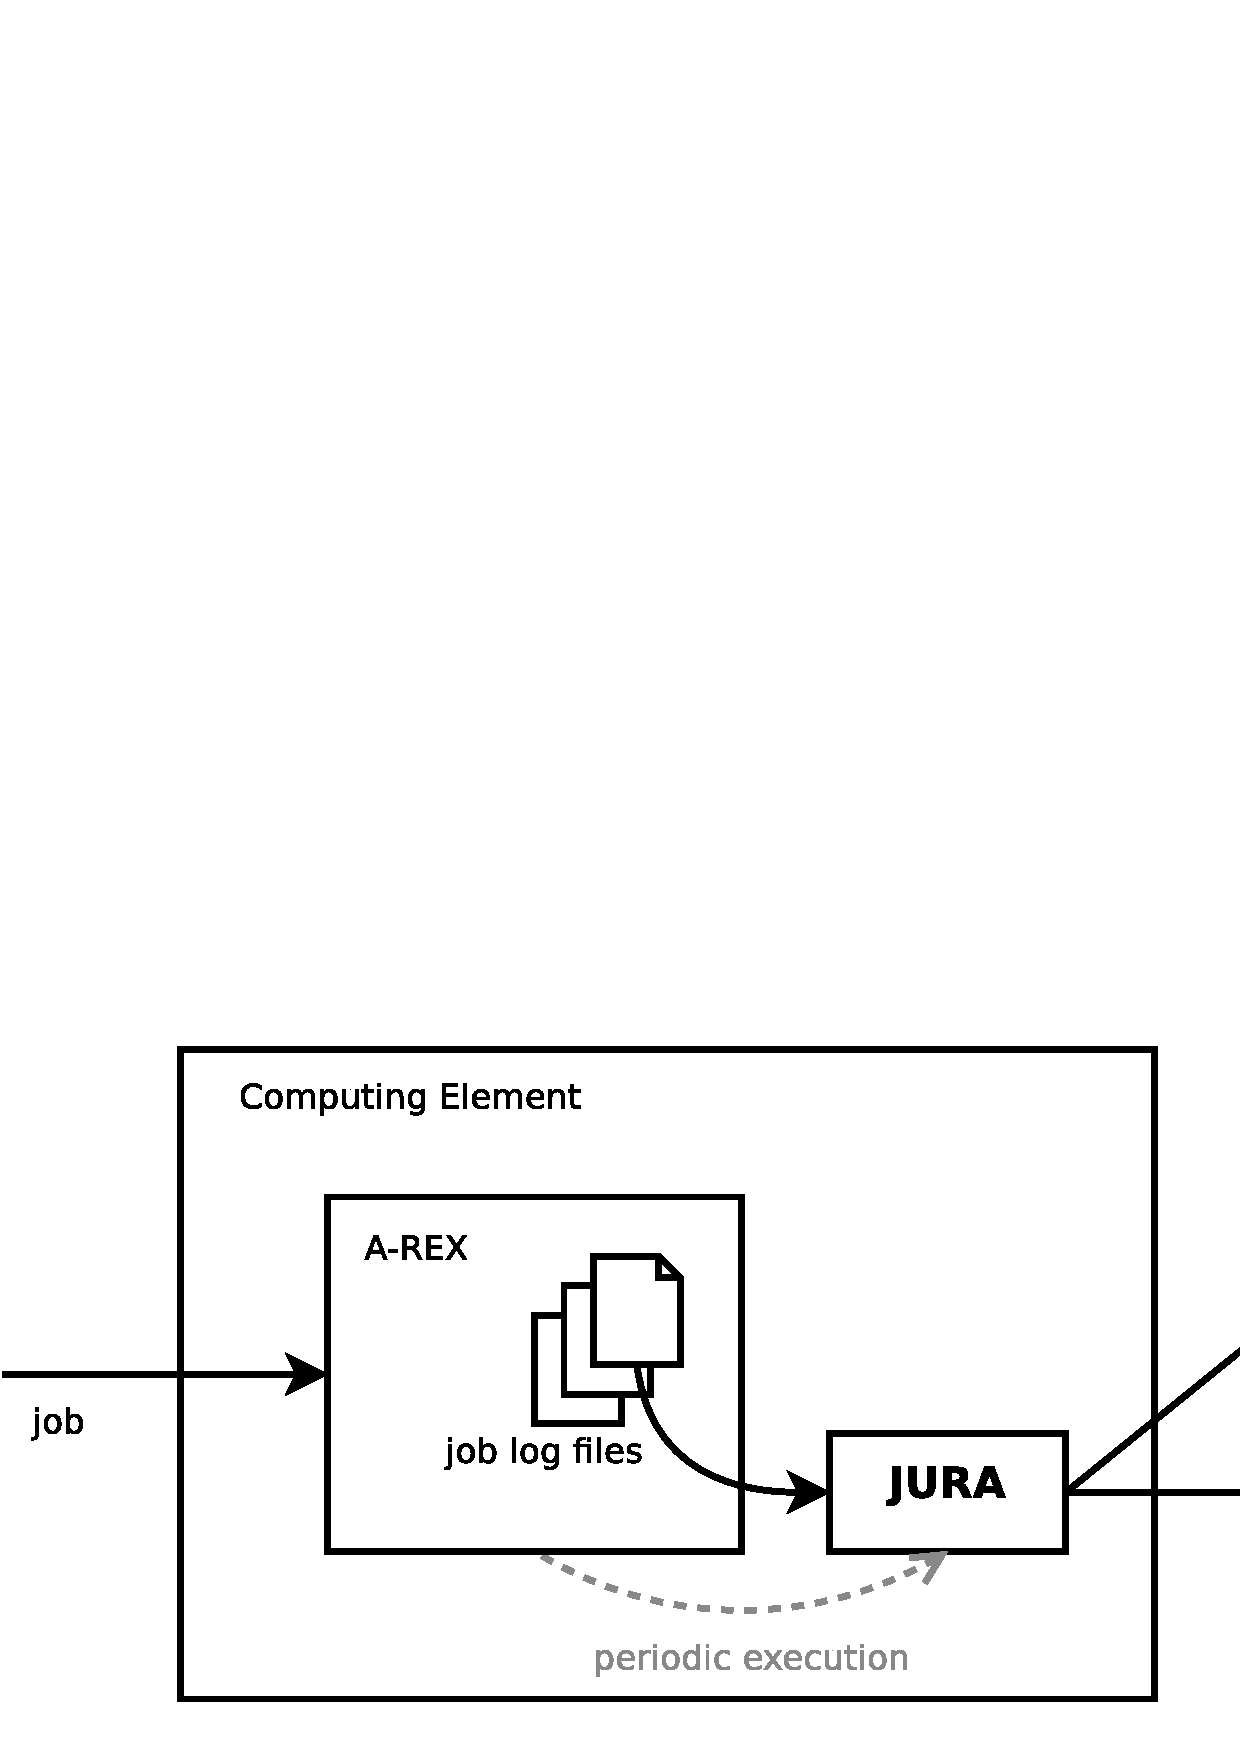
\includegraphics[width=0.9\textwidth]{components.pdf}}}
\caption{\label{fig:components}Components participating in accounting.} }
\end{figure}

JURA offers a complete replacement in functionality for the old
\textit{logger} utility\cite{logger}, a job metadata logging tool with
a purpose very closely related to that of this new tool. However,
backwards compatibility is maintained, so the old logger can still be
deployed.

The ARC execution manager, A-REX\cite{arex} initiates JURA in a
similar way to invoking logger. JURA reads job log files provided by
A-REX. These files have the same format as those meant for logger,
with additional lines which are necessary for accounting scenarios.

It also acts as a client for one or more accounting services,
specifically SGAS Logging and Usage Tracking Services (LUTS's),
inserting the generated records in batches. (See Figure
\ref{fig:components}.)

\section{Operation}

\subsection{Invocation}

JURA is a stand-alone executable application, executed hourly by
A-REX. It has no separate configuration file; it gets all necessary
configuration options from A-REX, in part through command-line
arguments, but mostly via lines in the job log files (see Appendix
\ref{config} for details). The source of the latter are lines in the
grid-manager configuration file.

The command line format is a subset of that of logger:

\verb|jura [-E <expiration_time>] <control_dir>|

where \textit{expiration\_time} is the validity length of job log
files in days, after which time they are considered invalid;
\textit{control\_dir} is the A-REX control directory for a mapped
local UNIX user.

\subsection{Parsing job log files}
\label{joblogs}
The job logs generated by A-REX reside under the directory
\verb|<control_dir>/logs|. They have file name format
\verb|<ngjobid>.<random>|, where \textit{ngjobid} is the identifier
created for the job by A-REX, \textit{random} is a randomly generated
sequence of alphanumeric characters to avoid collision of different
files pertaining to the same job.

2 for each logging destination: when submitted, when finished

UR generated from them: only from finished

\subsection{Accessing LUTS}

insert method

certificates from:...

\section{Security}
  runs as: same user as a-rex, typically root

  accesses sensitive data in job logs

  sgas security: 

    standard ssl cert, possibly proxy

    no other attributes but DN considered

    access control: flat-file based + XACML-like(?) configured thru
    SAM porttype

  in this case: service credentials, no proxy

\section{Implementation}
  c++

  sw dependencies

    full arc

    ssl

  install location

\appendix

\section{Configuration}
\label{config}
  jobreport

  jobreport\_options

  jobreport\_credentials

\section{Usage Record properties}
\label{log2ur}
  input file format

  filled properties

  missing properties

\bibliography{grid}
\end{document}
